
\documentclass[a4j,10pt]{jsarticle}
\usepackage{layout,url,resume}
\usepackage[dvipdfmx]{graphicx}
\pagestyle{empty}

\begin{document}
%\layout

\title{SMTP Strict Transport Security (SMTP-STS)
\\を用い暗号化された電子メール通信経路の確立とその実装}

% 和文著者名
\author{
    尾崎周也 (shuya) \thanks{慶應義塾大学 総合政策学部}
    \\shuya@sfc.wide.ad.jp
    \and
    親 中島博敬 (nunnun) \thanks{慶應義塾大学 政策・メディア研究科}
    \\nunnun@sfc.wide.ad.jp
}


% 和文概要
\begin{abstract}
\\SMTPはデファクトスタンダードのメール転送プロトコルであるが、MTA間の通信への中間者攻撃に脆弱性が存在する.本研究ではIETF UTA Working Groupで審議中のSMTP STS(SMTP Strict Transport Security)をJavaScriptで実装し既存実装との疎通を確認するとともに、その有用性と問題点を考察する.
\end{abstract}

\maketitle
\thispagestyle{empty}

\section{背景}

SMTPはWWW以前から使用され事実上の標準技術になっているメール配送プロトコルである.当初の仕様から今日に至るまで改善が続けられており現在も使用されている.電子メールは配送されるまでに幾つかのMTAを経由して配送されるが、その通信経路は必ずしも暗号化されていない.[図1]
\begin{figure}[htbp]
 \begin{center}
      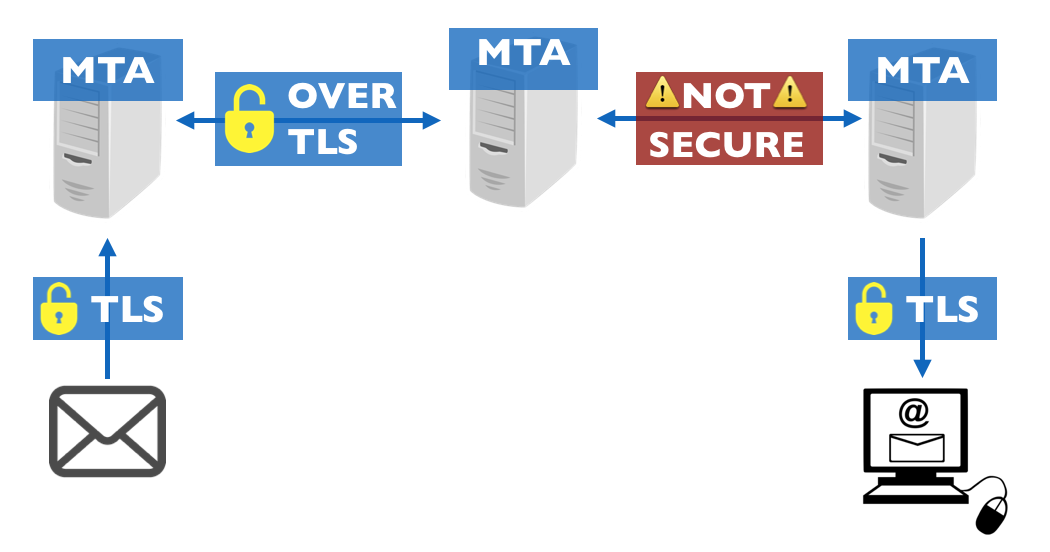
\includegraphics[width=7cm]{figure1.png}
      \caption{電子メールの配送経路}
    \end{center}
\end{figure}

つまり中間者攻撃には脆弱であり、以下に2つの攻撃例と図を記す.

\begin{itemize}
\item POODLE攻撃 
\item サーバの応答の正当性
\end{itemize}

POODLE攻撃とは通信のために古い暗号方式をサポートする対象に行われる攻撃だ.現在は暗号方式としてTLS1.2の使用が推奨されておりほとんどのサーバやブラウザはTLS1.2に対応している.しかし全てのサーバ、ブラウザが対応しているとは限らない.そのため互換性を確保するために古い暗号方式での通信リクエストを受ける場合がある.その際、SSL3.0のようなセキュリティホールが既知であるプロトコルで通信をすることが可能だ.このプロトコルのダウングレードを悪用して中間者攻撃を行うのがPOODLE攻撃である.

またサーバの応答の正当性をつく攻撃も考えられる.DNS応答が偽造・改竄されているサーバに接続した場合、ユーザは意図しない接続先に誘導される.DNSSECで正当性が証明されない限りそのサーバが意図したものかユーザは判断することができない.

\begin{figure}[htbp]
 \begin{center}
      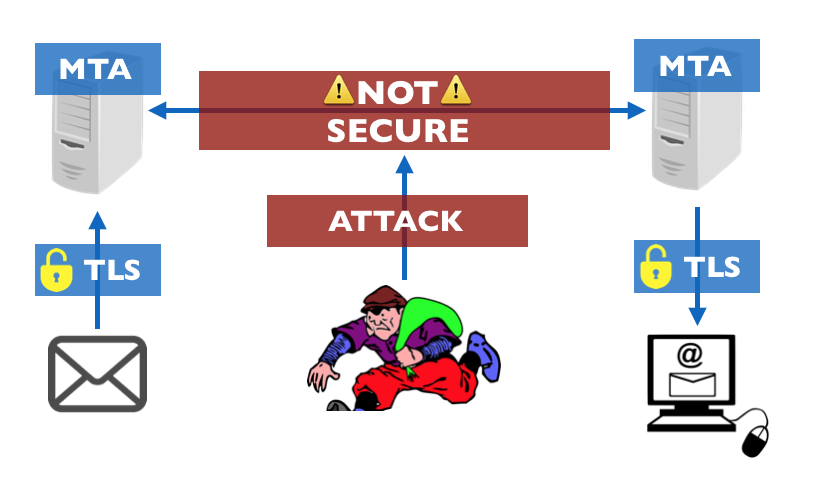
\includegraphics[width=5cm]{figure2.png}
      \caption{中間者攻撃例}
    \end{center}
\end{figure}


\section{研究目的}

本研究では中間者攻撃に脆弱であるSMTPプロトコルの現状を問題と考え、SMTP-STSによるセキュアなMTA間通信を実現することを目的としSMTP-STSをJavaScriptで実装する.



\section{関連技術}

関連技術としては以下の2点があげられる.
\begin{itemize}
\item HTTP Strict Transport Security (HSTS)
\item DNS-based Authentication of Named Entities(DANE)
\end{itemize}

HSTSはWebサーバがブラウザに対して現在のアクセス以降はHTTPではなくHTTPSでの接続を強制するセキュリティ機構である.SMTP-STSの考えはこれに基づくものだ.

DANEはドメイン(DNS)とそれに証明書を発行する証明局との紐付けを明確化するセキュリティ機構だ.DANEによってサーバの応答の正当性を担保することができる.

\section{SMTP-STS}

SMTP Strict Transport Security (SMTP-STS)はSMTPの中間者攻撃への脆弱性から検討されている新しいセキュリティ機構であり、IETF UTA Working Groupで審議中だ.\cite{draft}SMTP-STSの技術的特徴は2点に集約される.

\begin{itemize}
\item メールプロバイダが特定の認証(DANE)が有効なTLS接続上でメールの配送ができることを宣言する.
\item 通信経路が暗号化されていなかった場合は報告する、またはメールの受け取りを拒否する.
\end{itemize}

\section{実装}

実装は特定の機能、TLS接続のverifyの部分にしぼったMVPを実装する予定だ.また2つの方法を考えている.

\begin{enumerate}
\item Harakaプラグインとして実装する
\item 既存実装をJavaScriptで再実装する
\end{enumerate}

HarakaとはNode.jsで実装されたOSSのSMTPサーバであり、この拡張機能としての実装を目指す.既存実装を再実装するという点では、現在GitHub上にある実装物(go,pythonの2つ)は最新のドラフトを反映していないものであり、ドラフトを反映させた実装を目指す.

\section{評価}

評価は実装物と既存実装間で疎通がとれるかに設定する.またSMTP-STSを使用した・していない場合でのメール転送速度を計測する.

\section{展望}

先述したように本研究ではMVPのみの実装を行う.MVPのみを実装する理由はSMTP-STSの土台技術であるDNSSECが正常動作しているサーバが現時点ではまだ少ないためだ.\cite{dnssec}本研究のMVPと既存実装との疎通が確認された後、ドラフトに従いSMTP-STSの他の機能の実装を行う予定だ.

\begin{thebibliography}{9}
\bibitem{draft}
D. Margolis et al, “SMTP Strict Transport Security”, Internet Draft, March 2016.\\
\url{https://tools.ietf.org/html/draft-margolis-smtp-sts-01}

\bibitem{dnssec}
DNSSEC name and shame!\\
\url{ https://dnssec-name-and-shame.com/}
\end{thebibliography}

\end{document}
% end of file
